\documentclass[a4paper,12pt]{article} % тип документа
\usepackage{wrapfig}
\usepackage{tikz}
\usepackage[T2A]{fontenc}			% кодировка
\usepackage[utf8]{inputenc}			% кодировка исходного текста
\usepackage[english,russian]{babel}	% локализация и переносы
\usepackage{amsfonts,longtable}

% Математика
\usepackage{amsmath,amsfonts,amssymb,amsthm,mathtools} 


\usepackage{wasysym}

\title{Лабораторный журнал к работе 1.2.5 по курсу \\ "Общая физика"  \\ 
\vspace{0.2cm}
\vspace{4.5cm}
 \LARGE{\textbf{Исследование прецессии уравновешенного гироскопа}}\vspace{5.5cm}}
\date{07.12.2018}
\usepackage{tikz}
\author{\vspace{0.2cm}Баринов Леонид}

\begin{document}
\maketitle
\newpage
\textbf{Цель работы:} исследовать вынужденную прецессию гироскопа; установить зависимость скорости вынужденной прецессии от величины момента сил, действующих на ось гироскопа; определить скорость вращения ротора гироскопа и сравнить ее со скоростью, рассчитанной по скорости прецессии.

\textbf{В работе используются:} гироскоп в кардановом подвесе, секундомер, набор грузов, отдельный ротор гироскопа, цилиндр известной массы, крутильный маятник, штангенциркуль, линейка.

Уравнения движения твердого тела можно записать в виде:
\begin{equation}
\frac{\overrightarrow{P}}{dt} = \overrightarrow{F}
\end{equation}
\begin{equation}
\frac{d\overrightarrow{L}}{dt} = \overrightarrow{M}
\end{equation}
Здесь (1) выражает закон движения центра масс тела, а (2) — уравнение моментов. Поскольку твердое тело имеет только шесть степеней свободы, этих двух векторных уравнений достаточно для полного описания состояния его движения.

Если сила $\overrightarrow{F}$ не зависит от угловой скорости, а момент $\overrightarrow{M}$ — от скорости поступательного движения, то уравнения (1) и (2) можно рассматривать независимо друг от друга. В баллистике, например при движении снаряда в воздухе, это невозможно. В случае же, когда такое раздельное рассмотрение возможно, уравнение (1) соответствует просто задаче о движении материальной точки, а уравнение (2) — задаче о вращении твердого тела вокруг неподвижной точки. В данной работе рассматривается последняя из этих задач.

Момент импульса твердого тела в его главных осях$ х, у, z$ равен
\begin{equation}
\overrightarrow{L} = \overrightarrow{i}I_x\omega_x+\overrightarrow{j}I_y\omega_y + \overrightarrow{k}I_z\omega_z
\end{equation}
где $I_x, I_y, I_z$ — главные моменты инерции. usx, иу, u>z — компонента: вектора угловой скорости й. Быстро вращающееся тело, для которого, например,
\[I_z\omega_z \gg I_x\omega_x, I_y\omega_y\]
принято называть гироскопом. Гироскоп называется уравновешенным, если его центр масс неподвижен.

В силу (2) приращение момента импульса определяется интегралом
\begin{equation}
\Delta\overrightarrow{L} = \int\overrightarrow{M}dt
\end{equation}
Если момент внешних сил действует в течение короткого промежутка времени, из интеграла (4) следует, что приращение $\Delta\overrightarrow{L}$ момента импульса значительно меньше самого момента импульса:
\[|\Delta\overrightarrow{L}| \ll |\overrightarrow{L}|\]
С этим связана замечательная устойчивость, которую приобретает движение гироскопа после приведения его в быстрое вращение.
\begin{wrapfigure}{r}{0.5\textwidth}
  \begin{center}
    \includegraphics[width=0.48\textwidth]{1}
  \end{center}
  \caption{Маховик}
\end{wrapfigure}

Выясним, какие силы надо приложить к гироскопу, чтобы изменить направление его оси. Рассмотрим для примера маховик, вращающийся вокруг оси $z$, перпендикулярной к плоскости маховика (рис. 1). Будем считать, что
\[\omega_z = \omega_0, \quad \omega_x = 0, \quad \omega_y = 0.\]
Пусгь ось вращения повернулась в плоскости $zx$ по направлению к оси $х$ на бесконечно малый угол $d\varphi$. Такой поворот означает добавочное вращение маховика вокруг оси $y$, так что
\[d\varphi = \Omega dt,\]
где $\Omega$ — угловая скорость такого вращения. Будем предполагать, что
\begin{equation}
L_\Omega \ll L_{\omega_0}
\end{equation}
Это означает, что момент импульса маховика, равный $I_z\omega_0$ до приложения внешних сил, только повернется в плоскости $zx$ по направлению к оси $х$ не изменяя своей величины. Таким образом,
\[|d\overrightarrow{L}| = Ld\varphi = L\Omega dt\]
Но это изменение направлено вдоль оси $x$, поэтому вектор $d\overrightarrow{L}$ можно представить в виде векторного произведения вектора угловой скорости $\overrightarrow{\Omega}$, направленного вдоль оси $y$, на вектор собственного момента импульса маховика, направленного вдоль оси $z$,
\[d\overrightarrow{L} = \overrightarrow{\Omega} \times \overrightarrow{L}dt,\]
т. е.
\[\frac{d\overrightarrow{L}}{dt} = \overrightarrow{\Omega} \times \overrightarrow{L}\]
В силу (2) имеем
\begin{equation}
\overrightarrow{M} = \overrightarrow{\Omega} \times \overrightarrow{L}
\end{equation}
Формула (6) справедлива, если выполнено условие (5). Она позволяет определить момент сил $\overrightarrow{M}$, который необходимо приложить к маховику для того, чтобы вызвать вращение оси маховика с угловой скоростью $\overrightarrow{\Omega}$. Мы видим, таким образом, что для поворота оси вращающегося маховика к оси $x$ необходимо приложить силы, направленные не вдоль оси $x$, а вдоль оси $у$, так чтобы их момент $\overrightarrow{M}$ был направлен вдоль оси $x$.

Под действием момента $\overrightarrow{M}$ внешних сил ось гироскопа медленно вращается вокруг оси $у$ с угловой скоростью $\Omega$. Такое движение называется регулярной прецессией гироскопа. В частности, создающей момент внешней силой может оказаться сила тяжести, если центр масс гироскопа не совпадает с точкой подвеса. Для гироскопа массой $m_\text{г}$, у которого ось собственного вращения наклонена на угол $\alpha$ от вертикали, скорость прецессии, происходящей вокруг вертикальной оси под действием силы тяжести, равна
\begin{equation}
\Omega = \frac{M}{I_z\omega_0\sin\alpha}= \frac{m_\text{г}gl_\text{ц}\sin\alpha}{I_z\omega_0\sin\alpha} = \frac{m_\text{г}gl_\text{ц}}{I_z\omega_0}
\end{equation}
где $l_\text{ц}$ — расстояние от точки подвеса до центра масс гироскопа, т. е. скорость прецессии не зависит от угла $\alpha$.

Для изучения регулярной прецессии уравновешенного гироскопа к его оси подвешивают дополнительные грузы. Это смещает общий центр масс и создает момент сил тяжести, вызывающий прецессию. Скорость прецессии в этом случае равна
\begin{equation}
\Omega = \frac{mgl}{I_z\omega_0}
\end{equation}
где $m$ — масса груза, $l$— расстояние от центра карданова подвеса до точки крепления груза на оси гироскопа (рис. 3).

В данной работе исследуется регулярная прецессия уравновешенного гироскопа.

Уравновешенный гироскоп, закрепленный в кольцах карданова подвеса, показан на рис. 2. Наружное кольцо подвеса $\text{А}$ может свободно поворачиваться вокруг вертикальной оси $aa$. Внутреннее кольцо $\text{Б}$ связано с кольцом $\text{А}$ горизонтальной осью $\text{бб}$. В кольце $\text{Б}$ укреплен гироскоп, ось вращения которого $\text{вв}$ перпендикулярна к оси $\text{бб}$. Центр масс гироскопа находится на пересечении всех трех осей и при любом повороте колец сохраняет свое положение в пространстве. Получается, что гироскоп как бы подвешен за центр масс.
\begin{figure}[h]
\centering
\includegraphics[scale=0.5]{2}
\caption{Гироскоп в кардановом подвесе}
\end{figure}

Экспериментальная установка для исследования прецессии уравновешенного гироскопа показана на рис. 3. Ротором гироскопа является ротор высокооборотного электромотора $M$, питающегося током частотой $400\text{Гц}$. Кожух мотора (статор, имеющий обмотки, питаемые током частотой $400\text{Гц}$) скреплен с кольцом $\text{Б}$ (рис. 2 и 3). Мотор с кольцом $\text{Б}$ может вращаться в кольце $\text{А}$ вокруг горизонтальной оси $\text{бб}$, которое может вращаться вокруг вертикальной оси $\text{аа}$. Ротор электромотора представляет массивный стальной цилиндр с прожилками меди, образующими «беличье колесо». Обозначенный на рис. 3 буквой $\text{С}$ рычаг направлен по оси симметрии ротора. На рычаг подвешивают грузы $\text{Г}$. Подвешивая различные грузы, можно менять силу $F$, момент которой определяется расстоянием $I$ от точки подвеса до горизонтальной оси кольца $\text{А}$ (до центра масс гироскопа), указанным на самой установке.

Выше при выводе формул для прецессии предполагалось, что действующие на гироскоп силы лежат в плоскости $zy$, в которой лежат векторы угловых скоростей собственного вращения и прецессии. В этом случае, как уже говорилось, момент сил меняет лишь направление момента импульса гироскопа, но не его величину. Силы трения не лежат в плоскости осей вращения. Они приводят к изменению момента импульса и по направлению, и по величине. Для ротора гироскопа действие сил трения скомпенсировано действием электромотора. Для осей карданова подвеса компенсации нет. В результате ось гироскопа будет опускаться в направлении действия груза. 

В первой части работы исследуется зависимость скорости прецессии гироскопа от момента силы, приложенной к его оси. Для этого к оси гироскопа (к рычагу $\text{С}$) подвешиваются грузы $\text{Г}$. Скорость прецессии определяется по числу оборотов рычага вокруг вертикальной оси и вымени, которое на это ушло, определяемое секундомером. В процессе измерений рычаг не только поворачивается в результате прецессии гироскопа, но и опускается. Поэтому его в начале опыта следует приподнять на $5-6^\circ$. Опыт надо закончить, когда рычаг опустится на такой же угол.

Измерение скорости прецессии гироскопа позволяет вычислить угловую скорость вращения его ротора. Расчет производится по формуле (8). Момент инерции ротора относительно оси симметрии $I_0$ измеряется по крутильным колебаниям точной копии ротора, подвешиваемой вдоль оси симметрии на жесткой проволоке. Период крутильных колебаний $T_0$ зависит от момента инерции $I_0$ и модуля кручения проволоки $f$:
\begin{equation}
T_0 = 2\pi\sqrt{\frac{I_0}{f}}
\end{equation}

Чтобы исключить модуль кручения проволоки, вместо ротора гироскопа к той же проволоке подвешивают цилиндр правильной формы с известными размерами и массой, для которого легко можно вычислить момент инерции $I_\text{ц}$. Для определения момента инерции ротора гироскопа имеем
\begin{equation}
I_0 = I_\text{ц}\frac{T_0^2}{T_{\text{ц}}^2},
\end{equation}
здесь $T_\text{ц}$ -- период крутильных колебаний цилиндра.

Скорость вращения ротора гироскопа можно определить и не прибегая к исследованию прецессии. У используемых в работе гироскопов статор имеет две обмотки, необходимые для быстрой раскрутки гироскопа. В данной работе одну обмотку используют для раскрутки гироскопа, а вторую — для измерения числа оборотов ротора. Ротор электромотора всегда немного намагничен. Вращаясь, он наводит во второй обмотке переменную электродвижущую силу (ЭДС) индукции, частота которой равна частоте вращения ротора. Частоту этой ЭДС можно, в частности, измерить по фигурам Лиссажу, получаемым на экране осциллографа, если на один вход подать исследуемую ЭДС, а па другой — переменное напряжение с хорошо прокалиброванного генератора. При совпадении частот на экране получаем эллипс.\\
\textbf{Ход работы:} 
\begin{itemize}
\item[1] Установите ось гироскопа в горизонтальное положение, осторожно поворачивая ее за рычаг $\text{С}$.
\item[2] Включите питание гироскопа и подождите 4-5 минут, чтобы вращение ротора успело стабилизироваться.
\item[3] Убедитесь в том, что ротор вращается достаточно быстро: при легком постукивании по рычагу $\text{С}$ последний не должен изменять своего положения в пространстве. Объясните причину устойчивости оси гироскопа. «Поиграйте» с гироскопом, нажимая карандашом на рычаг $\text{С}$. Как движется гироскоп при нажатии на рычаг? По реакции гироскопа определите, в какую сторону вращается ротор.
\item[4]	Подвесьте к рычагу $\text{С}$ груз $\text{Г}$. При этом должна начаться прецессия гироскопа. Трение в оси (в какой именно?) приводит к тому, что рычаг $\text{С}$ начинает медленно опускаться.
\item[5] Отклоните рычаг $\text{С}$ на $5-6^{\circ}$ градусов вверх от горизонтальной плоскости. Подвесьте к нему груз $\text{Г}$ и с помощью секундомера найдите угловую скорость регулярной прецессии $\text{П}$ (по числу оборотов и времени прецессии). Измерения продолжайте до тех пор, пока рычаг $\text{С}$ не опустится на $5-6^{\circ}$ градусов ниже горизонтальной плоскости, сделав целое число оборотов относительно вертикальной оси. Измерьте также скорость опускания рычага $\text{С}$. Повторите этот опыт не менее пяти раз. Усредните полученные результаты.
\item[6] Проделайте всю серию экспериментов, описанных в пункте $5$ при $5-7$ значениях момента $\text{М}$ силы $F$ относительно центра масс гироскопа (длина плеча $l$ указана на установке). Результаты опытов изобразите в виде графика $\text{П}$ в зависимости от$\text{М}$.
\item[7]  Измерьте момент инерции ротора гироскопа относительно оси симметрии $I_0$. Для этого подвесьте ротор, извлеченный из такого же гироскопа, к концу вертикально висящей проволоки так, чтобы ось симметрии гироскопа была вертикальна, и измерьте период крутильных колебаний получившегося маятника. Замените ротор гироскопа цилиндром, для которого известны или легко могут быть измерены радиус и масса, и определите для него период крутильных колебаний. Пользуясь формулой (10), вычислите момент инерции ротора гироскопа $I_0$.
\item[8] Оцените погрешности в определении $I_0$ и $\Omega$.
\item[9] 	Рассчитайте с помощью (8) частоту вращения ротора гироскопа. 
\item[10] По скорости опускания рычага $\text{С}$ во время прецессии определите момент сил трения.
\item[11] 	Определите частоту вращения ротора гироскопа по фигурам Лиссажу. Для этого включите осциллограф и генератор тумблерами «Сеть» и подайте на «Вход Y» осциллографа сигнал со второй обмотки статора гироскопа (с двух клемм на подставке гироскопа), а на «Вход синхр.» — сигнал с выхода генератора. Для получения фигуры Лиссажу на осциллографе необходимо нажать тумблер «Вход X», повернуть вправо до упора ручку «Стабильность», переключателем «Усилитель U» добиться подходящего размера изображения по вертикали, а с помощью переключателя «Пределы шкалы U» и ручки «Рег. вых.» па генераторе — удобного размера изображения по горизонтали. 11ереключателем «Множитель частоты» и ручкой «Hz» на генераторе добейтесь, чтобы на экране осциллографа появилась фигура, похожая на эллипс. Подберите частоту генератора так, чтобы эллипс стал неподвижным. Если этого сделать не удается, то выключите на короткое время питание электромотора гироскопа, чтобы ток первой обмотки не наводил ЭДС во второй и не мешал измерениям. Делать измерения при этом надо быстро, так как при выключенном питании ротор гироскопа начинает замедлять свое вращение. Получение на экране осциллографа неподвижного эллипса означает, что частота сигнала генератора равна частоте вращения ротора гироскопа.
\item[12] 	Оцените погрешность полученных результатов. Сравните угловые скорости вращения ро тора гироскопа, определяемые разными методами.
\item[13] Убедитесь в применимости соотношения (5) в данной работе.

\end{itemize}
\end{document}